% QEC Edge Lab -- presentation (Junction Finland 2026)
% Build:  pdflatex qec_edge_lab.tex  (twice)
\documentclass[aspectratio=169,11pt]{beamer}
\usepackage[T1]{fontenc}
\usepackage{lmodern}
\usepackage{textcomp}
\usepackage{tikz}
\usetikzlibrary{arrows.meta,positioning,calc,shapes.geometric}
\usepackage{booktabs}
\usepackage{xcolor}
\usepackage{qrcode}

% ---- look (matches the demo video) ---------------------------------------------------------------
\definecolor{navy}{RGB}{10,31,77}
\definecolor{navy2}{RGB}{14,38,90}
\definecolor{accent}{RGB}{125,211,252}
\definecolor{green}{RGB}{52,211,153}
\definecolor{red}{RGB}{248,113,113}
\definecolor{dim}{RGB}{148,163,184}
\definecolor{pink}{RGB}{244,114,182}
\setbeamercolor{background canvas}{bg=navy}
\setbeamercolor{normal text}{fg=white}
\setbeamercolor{frametitle}{fg=white}
\setbeamercolor{title}{fg=white}
\setbeamercolor{subtitle}{fg=accent}
\setbeamercolor{author}{fg=dim}
\setbeamercolor{date}{fg=dim}
\setbeamercolor{itemize item}{fg=accent}
\setbeamercolor{itemize subitem}{fg=accent}
\setbeamercolor{footline}{fg=dim}
\setbeamerfont{frametitle}{series=\bfseries,size=\Large}
\setbeamerfont{title}{series=\bfseries,size=\huge}
\setbeamertemplate{navigation symbols}{}
\setbeamertemplate{itemize item}{\raisebox{0.15ex}{\tiny$\bullet$}}
\setbeamertemplate{frametitle}{%
  \vspace*{0.5em}\ifx\insertframesubtitle\empty\else{\color{accent}\scriptsize\bfseries\MakeUppercase{\insertframesubtitle}}\\[0.2em]\fi
  \insertframetitle}
\setbeamertemplate{footline}{\hfill{\color{dim}\tiny QEC Edge Lab \quad \insertframenumber\quad}\vspace{0.6em}}

\newcommand{\eur}{\texteuro}
\newcommand{\us}{\,$\mu$s}
\newcommand{\hl}[1]{{\color{accent}#1}}
\newcommand{\good}[1]{{\color{green}#1}}
\newcommand{\bad}[1]{{\color{red}#1}}
\newcommand{\dimnote}[1]{{\color{dim}\small #1}}
\newcommand{\bignum}[2]{{\color{#1}\fontsize{40}{44}\selectfont\bfseries #2}}
\newcommand{\shot}[2][\linewidth]{\includegraphics[width=#1]{figures/#2}}

\title{QEC Edge Lab}
\subtitle{A \eur60 Arduino that corrects real quantum-computer errors}
\author{Arduino UNO Q \;\textperiodcentered\; IBM Quantum \;\textperiodcentered\; on-device AI}
\date{Junction Finland 2026 \;\textperiodcentered\; The Green European Renaissance}

\begin{document}

% ==================================================================================================
\begin{frame}[plain]
  \begin{columns}[c]
    \column{0.55\textwidth}
      \titlepage
    \column{0.42\textwidth}
      \shot{board.jpg}\\[0.3em]
      \dimnote{Arduino UNO Q with the Modulino Knob and Buzzer}
  \end{columns}
\end{frame}

% ==================================================================================================
\begin{frame}{Quantum computers use qubits}\framesubtitle{Quantum computing in 30 seconds}
  \begin{columns}[c]
    \column{0.58\textwidth}
    \begin{itemize}\setlength\itemsep{0.8em}
      \item A normal bit is either 0 or 1.
      \item A qubit can hold a \hl{mix of 0 and 1}, and qubits can be linked together (entangled).
      \item That lets them simulate molecules and materials that overwhelm normal computers.
    \end{itemize}
    \column{0.38\textwidth}\centering
    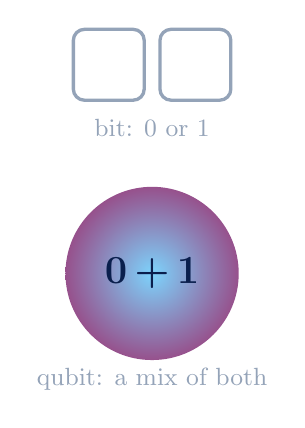
\begin{tikzpicture}
      \foreach \v/\x in {0/0,1/1.1}{\draw[dim,very thick,rounded corners] (\x,2.6) rectangle ++(0.9,0.9);
        \node[white,font=\Large\bfseries] at (\x+0.45,3.05) {\v};}
      \node[dim,font=\small] at (1,2.25) {bit: 0 or 1};
      \shade[inner color=accent,outer color=pink!60!navy] (1,0.4) circle (1.1);
      \node[navy,font=\Large\bfseries] at (1,0.4) {0\,+\,1};
      \node[dim,font=\small] at (1,-0.95) {qubit: a mix of both};
    \end{tikzpicture}
  \end{columns}
\end{frame}

% ==================================================================================================
\begin{frame}{Qubits make mistakes, constantly}\framesubtitle{The catch}
  \begin{columns}[c]
    \column{0.58\textwidth}
    \begin{itemize}\setlength\itemsep{0.8em}
      \item Heat, noise and time flip them by accident.
      \item Useful programs need millions of steps, so errors must be fixed on the fly.
      \item \hl{Error correction} spreads one bit over many qubits. A fast \hl{decoder} reads the clues and fixes the result.
    \end{itemize}
    \column{0.38\textwidth}\centering
    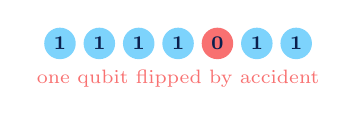
\begin{tikzpicture}
      \foreach \i in {0,...,6}{\pgfmathsetmacro\b{\i==4}
        \ifnum\i=4 \fill[red] (\i*0.5,0) circle (0.2); \node[navy,font=\scriptsize\bfseries] at (\i*0.5,0) {0};
        \else \fill[accent] (\i*0.5,0) circle (0.2); \node[navy,font=\scriptsize\bfseries] at (\i*0.5,0) {1}; \fi}
      \node[red,font=\scriptsize] at (1.5,-0.45) {one qubit flipped by accident};
    \end{tikzpicture}\\[1.2em]
    \bignum{white}{1 in 800}\\[0.3em]
    \dimnote{operations fail on IBM's best qubit pairs (ibm\_fez)}
  \end{columns}
\end{frame}

% ==================================================================================================
\begin{frame}{Shor's algorithm}\framesubtitle{The famous application}
  \begin{columns}[c]
    \column{0.58\textwidth}
    \begin{itemize}\setlength\itemsep{0.7em}
      \item Shor's algorithm (1994) factors huge numbers far faster than normal computers can.
      \item That breaks RSA and elliptic-curve encryption: the locks on banking, messaging and the power grid.
      \item It needs \hl{error correction}, with a fast decoder keeping up every round.
      \item \dimnote{So the EU wants critical infrastructure on quantum-safe encryption by 2030 [7].}
    \end{itemize}
    \column{0.38\textwidth}\centering
    
\begin{tikzpicture}
      \draw[red,line width=6pt] (-0.55,0.55) -- (-0.55,0.9) arc (180:0:0.55) -- (0.55,0.55);
      \fill[red,rounded corners=4pt] (-0.85,-0.6) rectangle (0.85,0.6);
      \fill[navy] (0,0.08) circle (0.15); \fill[navy] (-0.06,-0.35) rectangle (0.06,0.05);
    \end{tikzpicture}\\[0.6em]
    {\Huge\bfseries RSA-2048}\\[0.3em]
    \hl{$<$\,1 million noisy qubits, $<$\,1 week}\\
    \dimnote{estimate: Gidney, 2025 [6]}
  \end{columns}
\end{frame}

% ==================================================================================================
\begin{frame}{Why it matters for a greener Europe}\framesubtitle{The Green European Renaissance}
  \begin{columns}[c]
    \column{0.58\textwidth}
    \begin{itemize}\setlength\itemsep{0.6em}
      \item Design better \good{batteries} for electric cars and the power grid.
      \item Find cleaner \good{catalysts for fertiliser}: making ammonia uses about 1--2\% of the world's energy.
      \item Discover materials that \good{capture CO\textsubscript{2}}.
      \item \dimnote{Expected uses, still research: they all need error correction first.}
    \end{itemize}
    \column{0.38\textwidth}\centering
    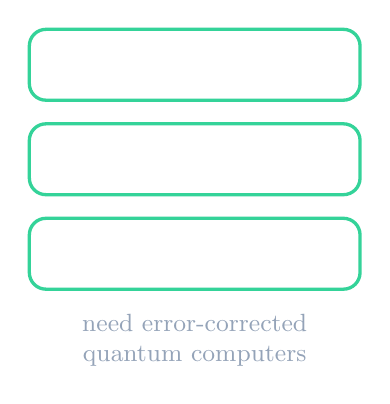
\begin{tikzpicture}[b/.style={draw=green,very thick,rounded corners=6pt,minimum width=4.2cm,minimum height=0.9cm,font=\large\bfseries,text=white}]
      \node[b] (a) at (0,2.2) {Batteries};
      \node[b] (b) at (0,1.0) {Clean fertiliser};
      \node[b] (c) at (0,-0.2) {CO\textsubscript{2} capture};
      \node[dim,font=\small,align=center] at (0,-1.3) {need error-corrected\\quantum computers};
    \end{tikzpicture}
  \end{columns}
\end{frame}

% ==================================================================================================
\begin{frame}{Big tech, big power}\framesubtitle{Today's decoders}
  \begin{columns}[c]
    \column{0.58\textwidth}
    \begin{itemize}\setlength\itemsep{0.7em}
      \item Google, IBM and NVIDIA decode on data-centre GPUs and FPGAs [1--5].
      \item \hl{Our idea:} a \eur60 European Arduino that learns each quantum chip's own errors, \hl{on the device}.
      \item \dimnote{To be fair: custom decoder chips use even less power ($\sim$8\,mW [9]), but cost millions and years to design.}
    \end{itemize}
    \column{0.38\textwidth}\centering
    \bignum{red}{700 W}\\ \dimnote{one data-centre GPU (NVIDIA H100) [10]}\\[1.2em]
    \bignum{green}{2--3 W}\\ \dimnote{the whole Arduino UNO Q [8]}
  \end{columns}
\end{frame}

% ==================================================================================================
\begin{frame}{What we built}\framesubtitle{One board, two computers}
  \centering
  \colorbox{white}{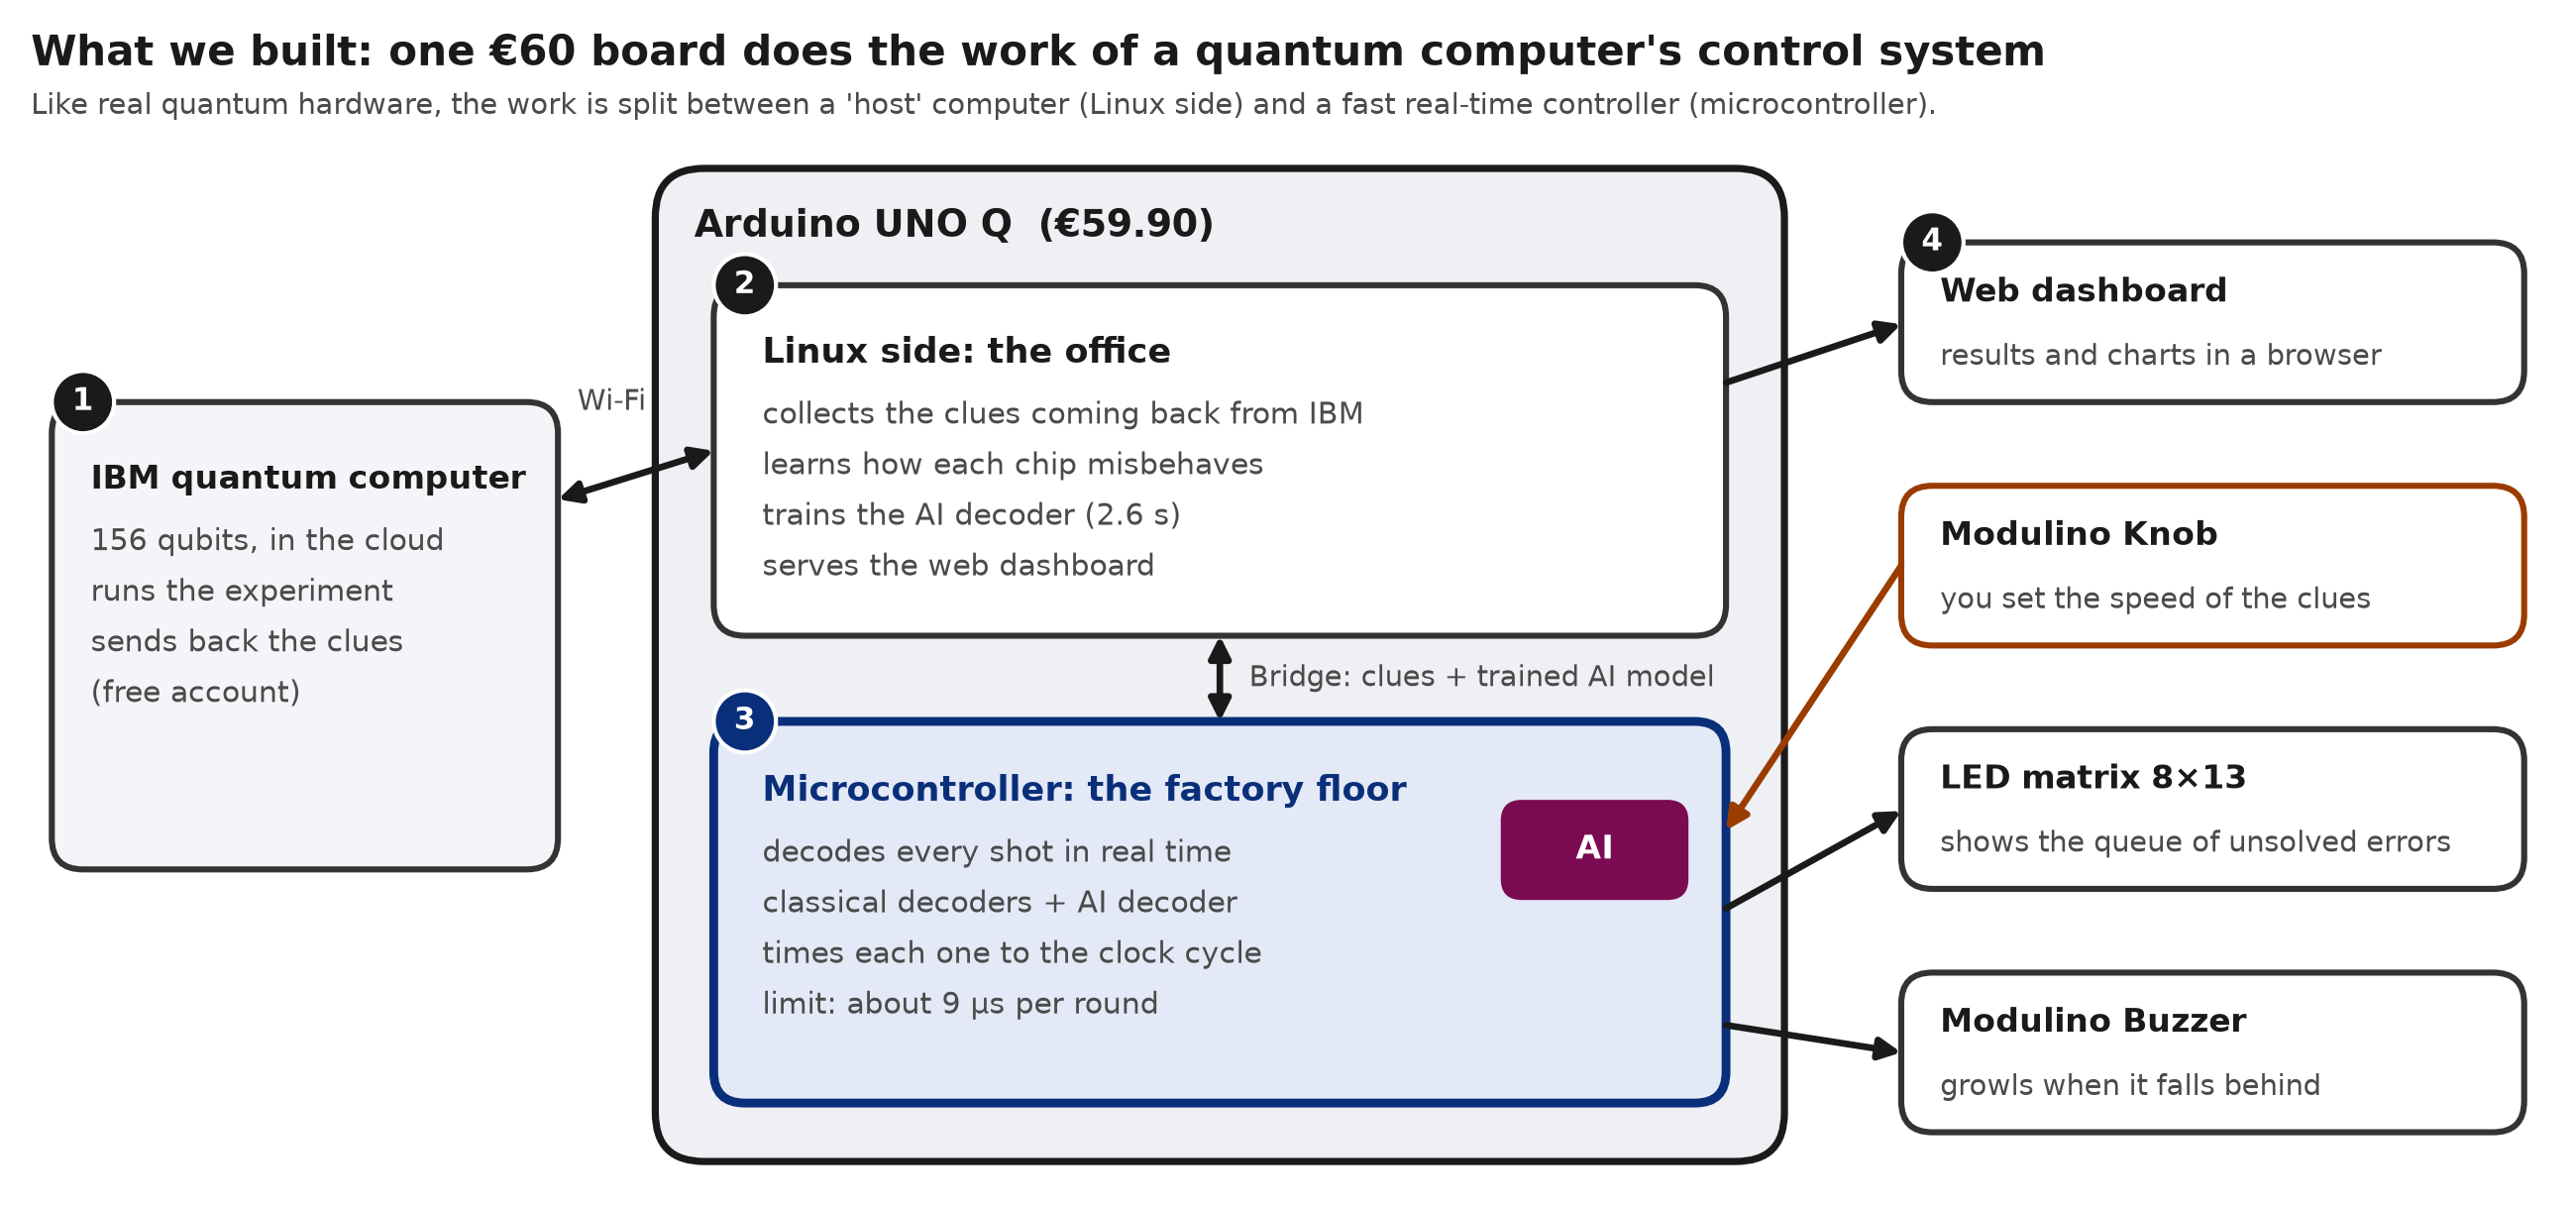
\includegraphics[width=0.9\textwidth]{figures/architecture.png}}
\end{frame}

% ==================================================================================================
\begin{frame}{How error correction works}\framesubtitle{The repetition code}
  \centering
  \colorbox{white}{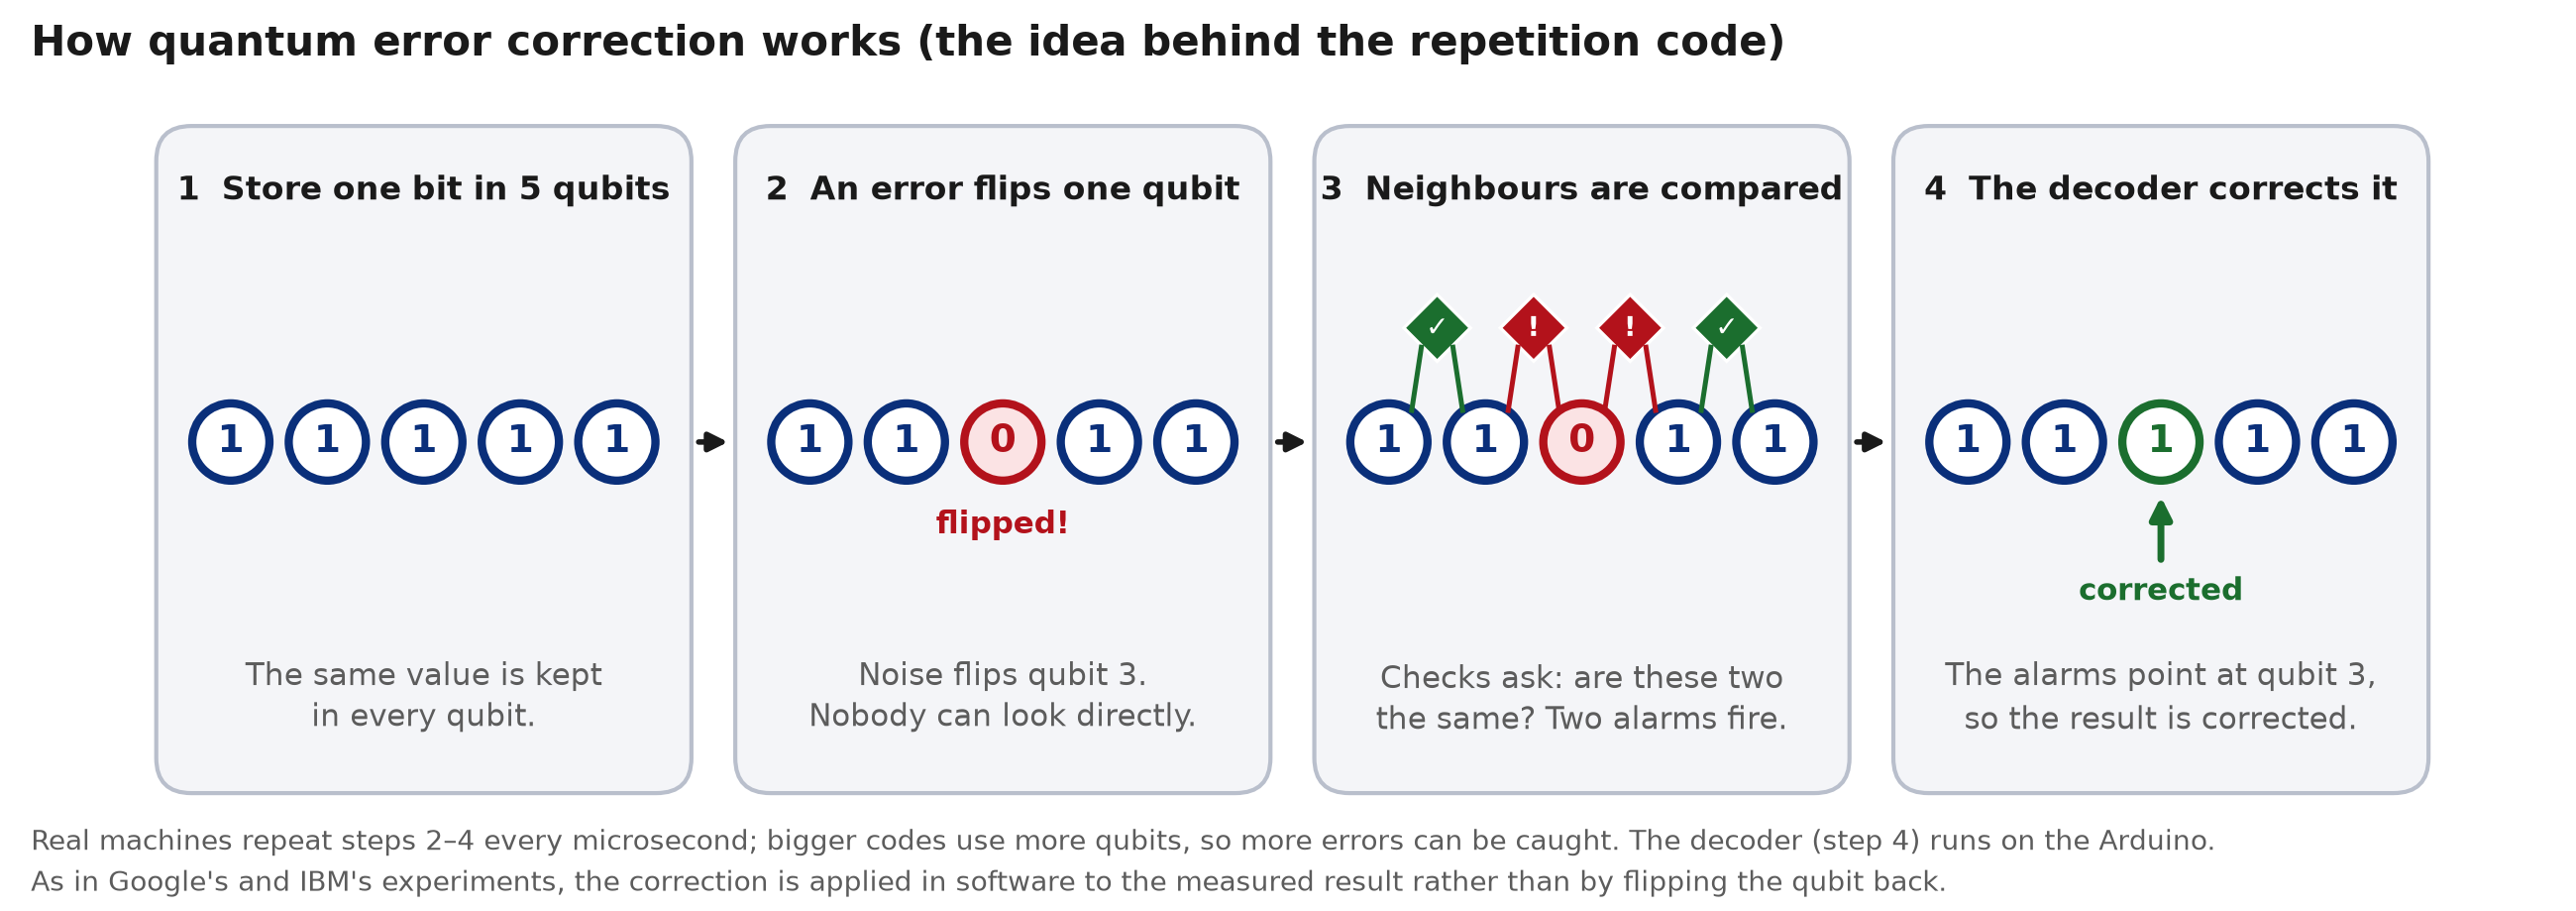
\includegraphics[width=0.93\textwidth]{figures/how_error_correction_works.png}}
\end{frame}

% ==================================================================================================
\begin{frame}{The QEC cycle: in theory and in practice}\framesubtitle{From textbook to bench}
  \centering
  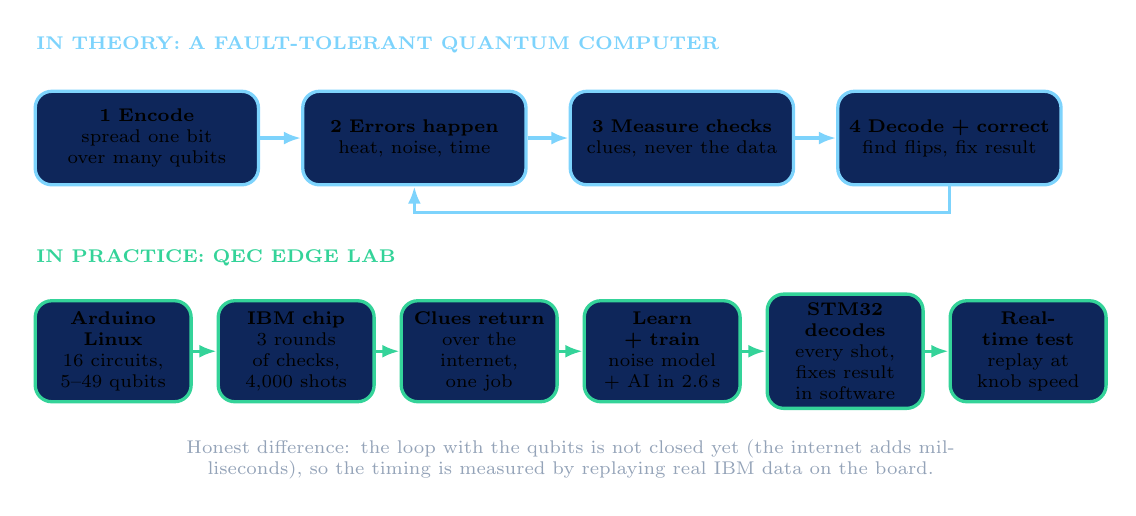
\begin{tikzpicture}[
      t/.style={draw=accent,very thick,rounded corners=6pt,fill=navy2,text width=2.75cm,align=center,minimum height=1.25cm,font=\scriptsize},
      p/.style={draw=green,very thick,rounded corners=6pt,fill=navy2,text width=1.85cm,align=center,minimum height=1.35cm,font=\scriptsize},
      a/.style={-{Latex[length=2.2mm]},very thick},scale=0.95,transform shape]
    \node[accent,font=\scriptsize\bfseries,anchor=west] at (-1.6,1.25) {IN THEORY: A FAULT-TOLERANT QUANTUM COMPUTER};
    \node[t] (t1) at (0,0) {\textbf{1 Encode}\\ spread one bit over many qubits};
    \node[t,right=0.55cm of t1] (t2) {\textbf{2 Errors happen}\\ heat, noise, time};
    \node[t,right=0.55cm of t2] (t3) {\textbf{3 Measure checks}\\ clues, never the data};
    \node[t,right=0.55cm of t3] (t4) {\textbf{4 Decode + correct}\\ find flips, fix result};
    \foreach \x/\y in {t1/t2,t2/t3,t3/t4} \draw[a,accent] (\x) -- (\y);
    \draw[a,accent] (t4.south) -- ++(0,-0.35) -| (t2.south);
    \node[font=\scriptsize,white] at ($(t2.south)!0.5!(t4.south)+(0,-0.62)$) {repeat every $\sim$1\us\ (superconducting) or $\sim$1\,ms (atoms, ions): the decoder must keep up};
    \begin{scope}[yshift=-2.85cm]
      \node[green,font=\scriptsize\bfseries,anchor=west] at (-1.6,1.25) {IN PRACTICE: QEC EDGE LAB};
      \node[p] (p1) at (-0.45,0) {\textbf{Arduino Linux}\\ 16 circuits, 5--49 qubits};
      \node[p,right=0.32cm of p1] (p2) {\textbf{IBM chip}\\ 3 rounds of checks, 4,000 shots};
      \node[p,right=0.32cm of p2] (p3) {\textbf{Clues return}\\ over the internet, one job};
      \node[p,right=0.32cm of p3] (p4) {\textbf{Learn + train}\\ noise model + AI in 2.6\,s};
      \node[p,right=0.32cm of p4] (p5) {\textbf{STM32 decodes}\\ every shot, fixes result in software};
      \node[p,right=0.32cm of p5] (p6) {\textbf{Real-time test}\\ replay at knob speed};
      \foreach \x/\y in {p1/p2,p2/p3,p3/p4,p4/p5,p5/p6} \draw[a,green] (\x) -- (\y);
      \node[dim,font=\scriptsize,text width=13cm,align=center] at ($(p1)!0.5!(p6)+(0,-1.45)$)
        {Honest difference: the loop with the qubits is not closed yet (the internet adds milliseconds), so the timing is measured by replaying real IBM data on the board.};
    \end{scope}
  \end{tikzpicture}
\end{frame}

% ==================================================================================================
\begin{frame}{Real quantum hardware, free account}\framesubtitle{IBM Quantum}
  \begin{columns}[t]
    \column{0.32\textwidth}\shot{ibm_job.jpg}\\[0.2em]\dimnote{Our job on ibm\_fez: 16 circuits, up to 49 qubits, $\sim$6\,s of QPU time}
    \column{0.32\textwidth}\shot{ibm_fez.jpg}\\[0.2em]\dimnote{IBM's live error rates: 156 qubits, best two-qubit error 1.2e-3}
    \column{0.32\textwidth}\shot{qubit_map.jpg}\\[0.2em]\dimnote{Every qubit is different, so the decoder must learn each chip}
  \end{columns}\vspace{0.6em}
  \begin{itemize}
    \item Bit-flip repetition codes, distance 3--25, 3 rounds of mid-circuit measurement, logical $|0\rangle$ and $|1\rangle$.
    \item Chips: ibm\_fez, ibm\_marrakesh (Heron r2, 156 qubits). A SWAP-free line of qubits is found automatically.
  \end{itemize}
\end{frame}

% ==================================================================================================
\begin{frame}{Edge AI: the Arduino trains its own decoder}\framesubtitle{On-device AI}
  \begin{columns}[c]
    \column{0.57\textwidth}
    \small
    \begin{itemize}\setlength\itemsep{0.35em}
      \item \hl{Trained in plain numpy} on the board's Linux side: $\sim$2.6\,s per model, no GPU, no cloud.
      \item Small network: clues + final readout $\to$ 32 neurons $\to$ ``flip or not''.
      \item Weights become 15-bit integers; the STM32 runs it with \hl{additions only}, bit-exact with Python, $\sim$8.5\,KB RAM.
      \item \hl{Honest test:} scored only on shots it never saw (2-fold cross-fitting); the right answer is never an input.
      \item \hl{Why it wins:} a stored 1 decays to 0 roughly 3--20$\times$ more often than the reverse (depends on chip and qubit). The AI learned this by itself.
    \end{itemize}
    \column{0.40\textwidth}
    \shot{ai_result.jpg}\\[0.2em]\dimnote{Dashboard: the AI decoder (pink) vs classical decoders}
  \end{columns}
\end{frame}

% ==================================================================================================
\begin{frame}{Results on real IBM quantum computers}\framesubtitle{Results}
  \begin{columns}[c]
    \column{0.52\textwidth}\centering
    \colorbox{white}{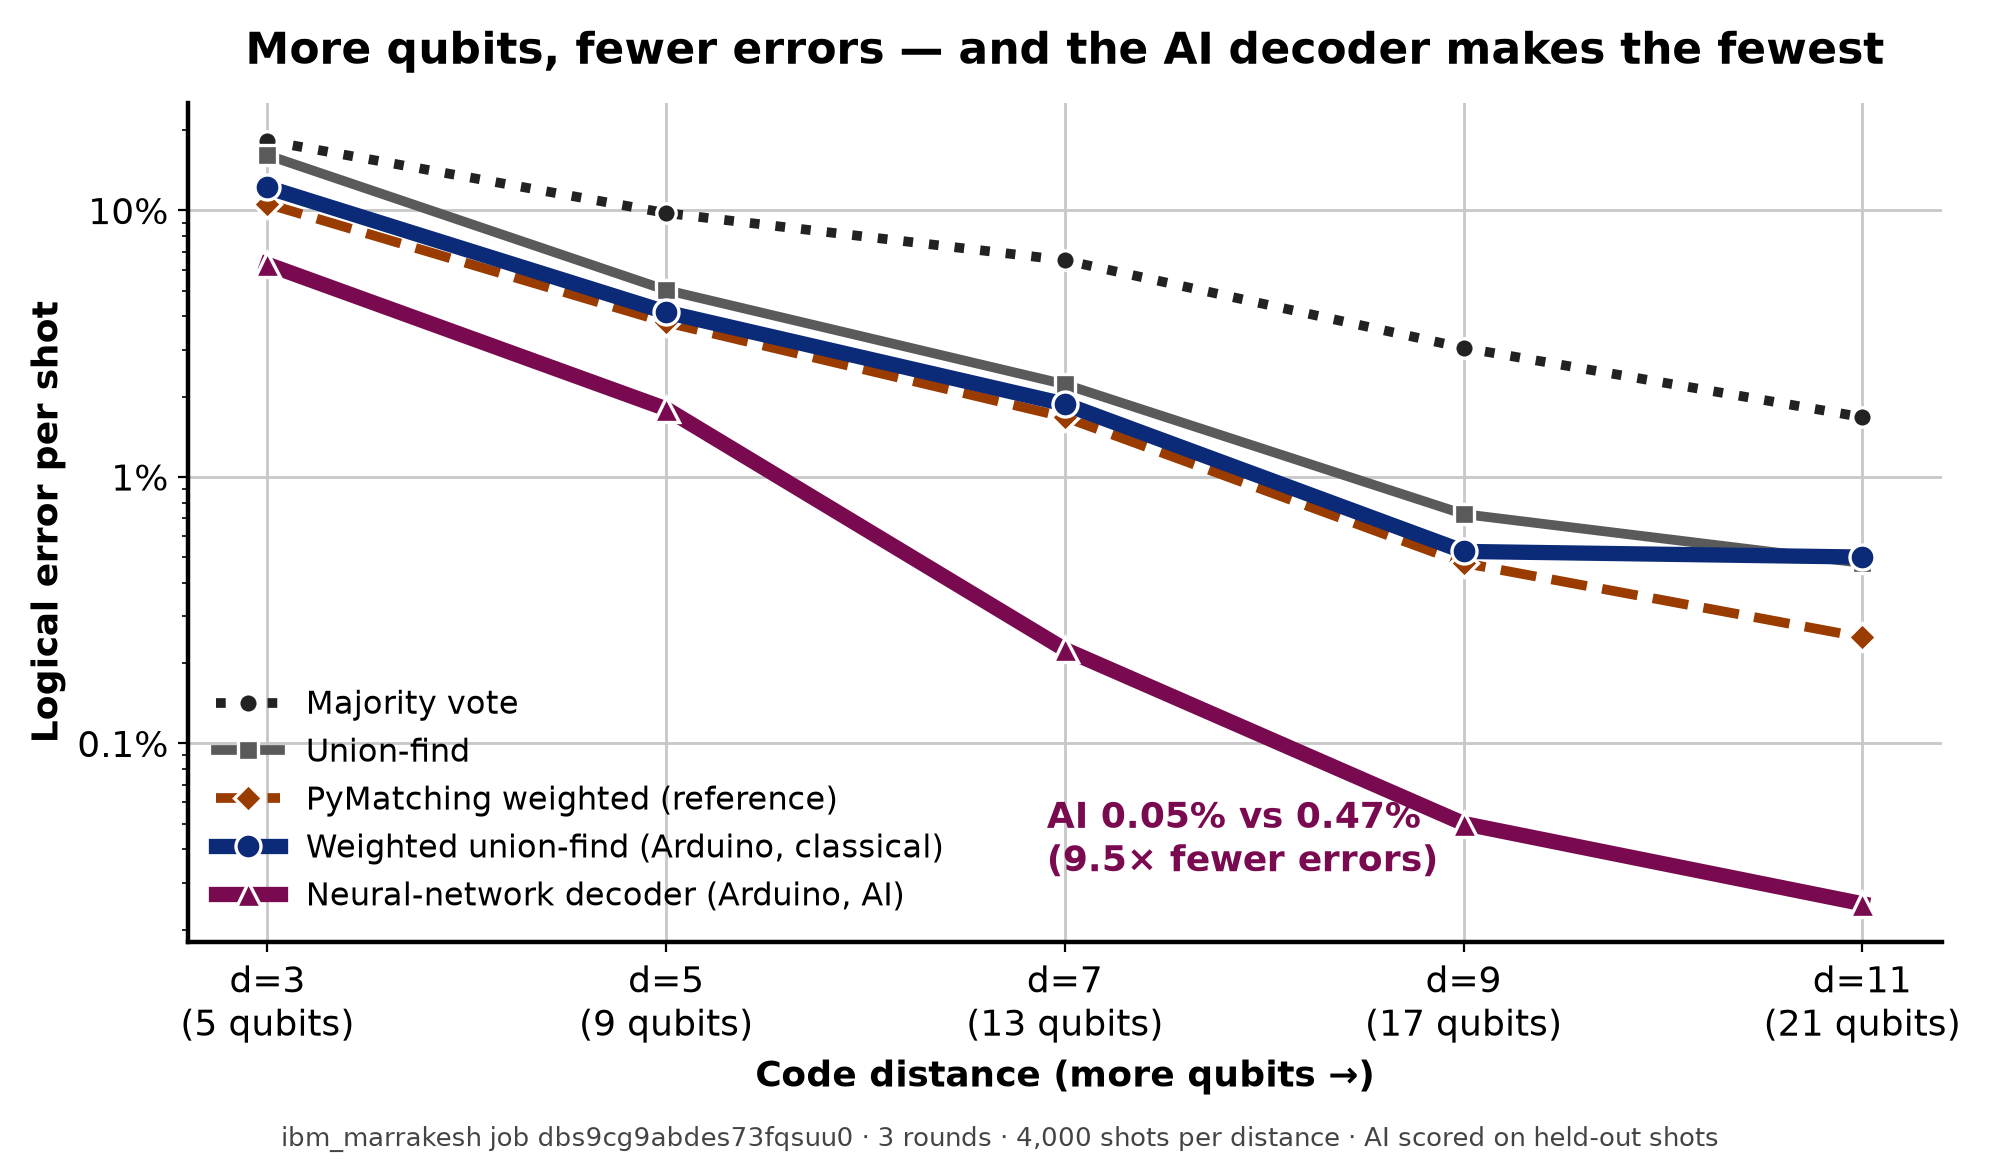
\includegraphics[width=0.93\linewidth]{figures/logical_error_vs_distance_ibm_marrakesh.png}}\\[0.6em]
    {\scriptsize
    \begin{tabular}{lcc}\toprule
      ibm\_marrakesh & best graph decoder & \textbf{AI} \\\midrule
      9 qubits (d=5) & 3.6\% & \textbf{1.8\%} \\
      13 qubits (d=7) & 1.7\% & \textbf{0.22\%} \\
      17 qubits (d=9) & 0.47\% & \textbf{0.05\%} \\\bottomrule
    \end{tabular}}
    \column{0.45\textwidth}
    \small
    \begin{itemize}\setlength\itemsep{0.5em}
      \item \good{Error correction works:} on ibm\_fez, 5 $\to$ 21 qubits cut mistakes from 4.8\% to 0.075\% (64$\times$).
      \item \good{AI decoder:} up to 9.5$\times$ fewer errors (typically 2--3$\times$) than the best classical decoder: up to 17 qubits on ibm\_marrakesh, up to 13 on ibm\_fez.
      \item The Arduino found a qubit that flips 31\% of the time.
      \item Classical union-find made 1.6--4$\times$ faster on the STM32, identical answers.
    \end{itemize}
  \end{columns}
\end{frame}

% ==================================================================================================
\begin{frame}{Turn the knob: can the Arduino keep up?}\framesubtitle{Real time, physical}
  \begin{columns}[t]
    \column{0.32\textwidth}\shot{knob.jpg}\\[0.2em]\dimnote{Modulino Knob sets how fast new clues arrive}
    \column{0.32\textwidth}\shot{led_matrix.jpg}\\[0.2em]\dimnote{LED matrix: the queue of unsolved errors}
    \column{0.32\textwidth}\shot{falling_behind.jpg}\\[0.2em]\dimnote{Too fast: the decoder falls behind; the buzzer growls}
  \end{columns}\vspace{0.4em}
  {\scriptsize\centering
  \begin{tabular}{lccc}\toprule
    STM32, ibm\_marrakesh, d=5 & mean decode & \textbf{limit per round} & kept up / fell behind \\\midrule
    AI decoder & 26.0\us & \textbf{8.7\us} & 10\us\ / 5.6\us \\
    Union-find weighted & 25.9\us & 8.6\us & 10\us\ / 5.6\us \\
    Union-find fast & 31.0\us & 10.4\us & 17.8\us\ / 10\us \\
    Union-find naive & 59.3\us & 19.8\us & 31.6\us\ / 17.8\us \\\bottomrule
  \end{tabular}\par}
\end{frame}

% ==================================================================================================
\begin{frame}{Decoders for the quantum computers Europe builds}\framesubtitle{Built for Europe}
  \begin{columns}[c]
    \column{0.58\textwidth}
    \begin{itemize}\setlength\itemsep{0.7em}
      \item Atom and ion quantum computers take about 1\,ms per round: \good{100$\times$ more time} than our Arduino needs [11,12].
      \item Open source; the decoder and its AI run locally, with no cloud AI service.
      \item The EU Quantum Europe Strategy aims for quantum leadership by 2030 [13].
      \item \dimnote{Next: test on atom and ion machines, and measure the board's power.}
    \end{itemize}
    \column{0.38\textwidth}\centering
    \bignum{green}{100$\times$}\\ \dimnote{more time per round on atom and ion machines}\\[1em]
    {\color{accent}\bfseries Europe's quantum builders}\\[0.3em]
    {\small Pasqal \textperiodcentered{} France \textperiodcentered{} atoms\\
    planqc \textperiodcentered{} Germany \textperiodcentered{} atoms\\
    AQT \textperiodcentered{} Austria \textperiodcentered{} ions\\
    IQM \textperiodcentered{} Finland \textperiodcentered{} superconducting}
  \end{columns}
\end{frame}

% ==================================================================================================
\begin{frame}{Honest limitations}\framesubtitle{What we have not shown}
  \begin{itemize}\setlength\itemsep{0.6em}
    \item \textbf{Emulated real time:} real IBM data replayed on the STM32; timing is real, the loop with the qubits is not closed.
    \item \textbf{Too slow for superconducting qubits} ($\sim$9\us\ vs $\sim$1\us\ per round); likely fast enough for atoms and ions.
    \item \textbf{Correction in software, after the run}, as in Google's and IBM's memory experiments (Pauli-frame tracking).
    \item \textbf{Repetition code only:} bit flips, not phase errors; 2-D codes (surface, colour) are next.
    \item \textbf{AI error floor} of 0.2--0.3\% on large codes, where classical decoders win: best design uses both.
    \item \textbf{Energy and impact are projections:} board power not yet measured during our runs; impact is indirect and long-term.
  \end{itemize}
\end{frame}

% ==================================================================================================
\begin{frame}{Try it}\framesubtitle{Links}
  \begin{columns}[c]
    \column{0.66\textwidth}
    {\Large\bfseries A few watts, open, European:\\[0.2em] \hl{decoders for Europe's quantum computers}}\\[1.4em]
    {\small
    \dimnote{Interactive demo}\\ \hl{victor-onofre.github.io/QEC\_Edge\_Lab\_submission}\\[0.6em]
    \dimnote{Code and data}\\ \hl{github.com/victor-onofre/QEC\_Edge\_Lab\_submission}\\[0.6em]
    \dimnote{Hardware and software}\\ Arduino UNO Q (\eur59.90), Modulino Knob and Buzzer, App Lab, Qiskit, IBM Quantum (free plan), numpy}
    \column{0.3\textwidth}\centering
    \colorbox{white}{\color{black}\qrcode[height=3.4cm]{https://victor-onofre.github.io/QEC_Edge_Lab_submission/demo/}}\\[0.5em]
    \dimnote{Scan: interactive demo}
  \end{columns}
\end{frame}

% ==================================================================================================
\begin{frame}[allowframebreaks]{References}
  \tiny
  \begin{enumerate}\setlength\itemsep{0.15em}
    \item Riverlane, decoders as ``the beating heart of QEC''. \url{https://www.riverlane.com}
    \item Google Quantum AI, Quantum error correction below the surface code threshold, Nature (2024).
    \item Bausch et al. (Google DeepMind), Learning high-accuracy error decoding for quantum processors (AlphaQubit), Nature (2024).
    \item NVIDIA, CUDA-Q QEC 0.6 with NVQLink (2026). \url{https://nvidia.github.io/cuda-quantum/blogs/blog/2026/04/14/cudaq-qec-0.6/}
    \item IBM Quantum, Real-time decoding of the gross code memory with FPGAs, arXiv:2510.21600.
    \item C. Gidney, How to factor 2048 bit RSA integers with less than a million noisy qubits, arXiv:2505.15917 (2025).
    \item NIS Cooperation Group, A coordinated implementation roadmap for the transition to post-quantum cryptography (2025).
    \item J. Geerling, The Arduino Uno Q is a weird hybrid SBC (power: $\sim$0.5\,W idle, 2--3\,W full load).
    \item Barber et al. (Riverlane), A real-time, scalable, fast and highly resource efficient decoder for a quantum computer, arXiv:2309.05558.
    \item NVIDIA H100 Tensor Core GPU datasheet (SXM: up to 700\,W).
    \item Bluvstein et al. (Harvard, QuEra, MIT), A fault-tolerant neutral-atom architecture for universal quantum computation, Nature (2025).
    \item Quantinuum Helios logical memory with neural-network decoders (Quantum Computing Report).
    \item European Commission, Quantum Europe Strategy (2 July 2025).
  \end{enumerate}
\end{frame}

\end{document}
